\documentclass{beamer}

\usetheme{CambridgeUS}
\usecolortheme{whale}
\usepackage[utf8]{inputenc}
\usepackage[T1]{fontenc}
\usepackage[french]{babel}
\usepackage{graphicx}
\usepackage{hyperref}
\usepackage{bookmark}
\usepackage{amsmath, amsfonts}
\setbeamertemplate{navigation symbols}{}
\useoutertheme{shadow}
\setbeamercolor{frametitle}{fg=white, bg=blue!30!black}
\setbeamercolor{section in head/foot}{fg=white,bg=blue!30!black}
\setbeamercolor{section in head/foot shaded}{fg=gray!70,bg=blue!30}
\setbeamercolor{subsection in head/foot}{fg=white,bg=blue!40!black}
\setbeamercolor{subsection in head/foot shaded}{fg=gray!50,bg=blue!10}
\setbeamertemplate{frametitle}[default]


\graphicspath{{../Saves/}}

\title[TIPE - Cycles et Boucles]{Analyse du sommeil à l'aide de l'Inteligence Artificielle}
\author{Ewann Roche / numéros candidat: XXXXXXX}
\date{\today}

\begin{document}

{
  \setbeamertemplate{headline}{%
    \leavevmode
    \hbox{%
      \begin{beamercolorbox}[wd=\paperwidth,ht=2ex,dp=2ex]{section in head/foot}
      \end{beamercolorbox}%
    }%
  }
  \begin{frame}
    \titlepage
  \end{frame}
}

\begin{frame}[plain]{Plan de la présentation}

  \vspace*{2.3cm}
  \begin{center}
    \tableofcontents
  \end{center}
  \vspace{0.5cm}

  \vspace*{2.5cm}
  \begin{beamercolorbox}[wd=\paperwidth,ht=2ex,dp=0.1ex,center]{author in head/foot}
    \usebeamertemplate*{footline}
  \end{beamercolorbox}
\end{frame}

\section{Introduction}

\begin{frame}{Problématique}
  \begin{block}{Contexte}
    L'analyse du sommeil est un enjeu de santé crucial et croissant.
  \end{block}

  \begin{block}{Question centrale}
     l'IA peut-elle prédire la qualité du sommeil et identifier d'éventuels troubles à partir de données accessibles ?
  \end{block}

  \begin{block}{Mon approche}
    Développement et adaptation de modèles d'IA (classification binaire et multiclasse) pour ces tâches
  \end{block}
\end{frame}

\section{Contexte et données}

\begin{frame}{Le thème : Cycles et Boucles}
    \centering
    Cycles biologiques : sommeil, rythme circadien\\
    \vspace{0.5cm}
    Boucles dans l'IA : entraînement itératif, rétropropagation\\
    \vspace{0.5cm}
    Boucle utilisateur : collecte → IA → retour personnalisé\\
\end{frame}


\begin{frame}{Présentation du dataset}
    \centering
    \vspace{1cm}
    Source : \href{https://www.kaggle.com/datasets/uom190346a/sleep-health-and-lifestyle-dataset}{Kaggle - Sleep Health and Lifestyle Dataset}\\
    \vspace{0.5cm}
    374 entrées, 13 variables\\
    \vspace{0.5cm}
    \begin{block}{Exemples de variables}
        \begin{itemize}
          \item Age, Sexe, Durée de sommeil
          \item Niveau de stress, Activité physique
          \item Fréquence cardiaque, Tension artérielle
        \end{itemize}
    \end{block}
\end{frame}

\begin{frame}{Prétraitement des données}
  \begin{block}{Nettoyage}
       Gestion des valeurs manquantes et retrait de colone inutile.
  \end{block}
  \begin{block}{Encodage}
      Transformation des variables vers des valeurs numériques
  \end{block}
  \begin{block}{Normalisation}
      Transformation des données selon une échelle, ici un échelle logique
  \end{block}
\end{frame}

\section{Modélisation IA}

\begin{frame}{Modèles IA utilisés}
    \begin{block}{Modèles}
        \begin{itemize}
          \item \textbf{Regresion} : valeur de qualité du sommeil (en pourcentage)
          \item \textbf{Multiclasse} : Détecter des troubles spécifiques (insomnie, apnée, ou aucun trouble).
        \end{itemize}
    \end{block}
    \begin{block}{Architecture commune}
        \begin{itemize}
            \item Réseau de neurones multicouches (MLP) : Flexibilité pour différents types de sorties.
            \item Implémentation : Classe Python modulaire et réutilisable.
        \end{itemize}
    \end{block}
\end{frame}

\begin{frame}{Extrait du template Python}
  \begin{center}
    \includegraphics[width=0.9\textwidth]{screen_class.png}
  \end{center}
\end{frame}

\section{Résultats et interface}

\begin{frame}{Courbes d'apprentissage}
    \begin{center}

      \begin{minipage}{0.7\linewidth}
        \centering
        \includegraphics[width=\linewidth]{curve_sleep_quality.png}
      \end{minipage}

      \begin{minipage}{0.7\linewidth}
        \centering
        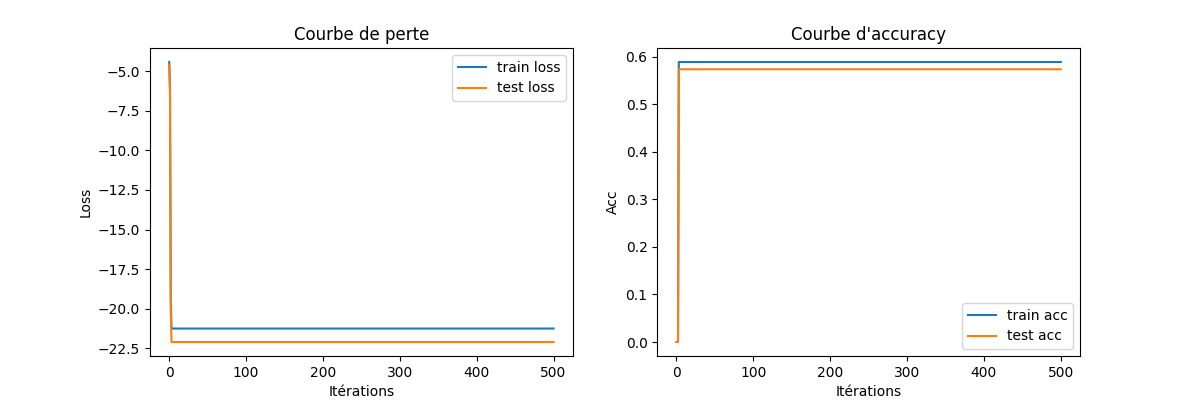
\includegraphics[width=\linewidth]{curve_sleep_trouble.png}
      \end{minipage}
      
    \end{center}
\end{frame}


\begin{frame}{Métriques de performance : Définitions}
    \begin{block}{Régression}
        \begin{itemize}
            \item \textbf{\boldmath$R^2$} : Coefficient de détermination.
            \item \textbf{MSE} : Erreur Quadratique Moyenne (Mean Squared Error).
            \item \textbf{MAE} : Erreur Absolue Moyenne (Mean Absolute Error).
        \end{itemize}
    \end{block}

    \begin{block}{Classification}
        \begin{itemize}
            \item \textbf{Accuracy} : Proportion de prédictions correctes.
            \item \textbf{Précision} : Proportion de vrais positifs parmi les prédictions positives.
            \item \textbf{Rappel} : Proportion de vrais positifs parmi les positifs réels.
            \item \textbf{F1-score} : Moyenne harmonique de la Précision et du Rappel.
        \end{itemize}
    \end{block}
\end{frame}


\begin{frame}{Métriques de performance : Résultats}
    \begin{block}{Modèle de Régression (Qualité du Sommeil)}
        \begin{itemize}
            \item \textbf{Entraînement} : $R^2 = 0.7962$, MSE = $0.0028$, MAE = $0.0245$
            \item \textbf{Test} : $R^2 = 0.7879$, MSE = $0.0032$, MAE = $0.0267$
        \end{itemize}
    \end{block}

    \begin{block}{Modèle de Classification Multiclasse (Troubles du Sommeil)}
        \begin{itemize}
            \item \textbf{Entraînement} : Accuracy = $0.8796$, F1-score = $0.8801$, Précision = $0.8522$, Rappel = $0.8796$
            \item \textbf{Test} : Accuracy = $0.8533$, F1-score = $0.8522$, Précision = $0.8816$, Rappel = $0.8533$
        \end{itemize}
    \end{block}
\end{frame}


\begin{frame}{Interface utilisateur}
  \begin{center}
    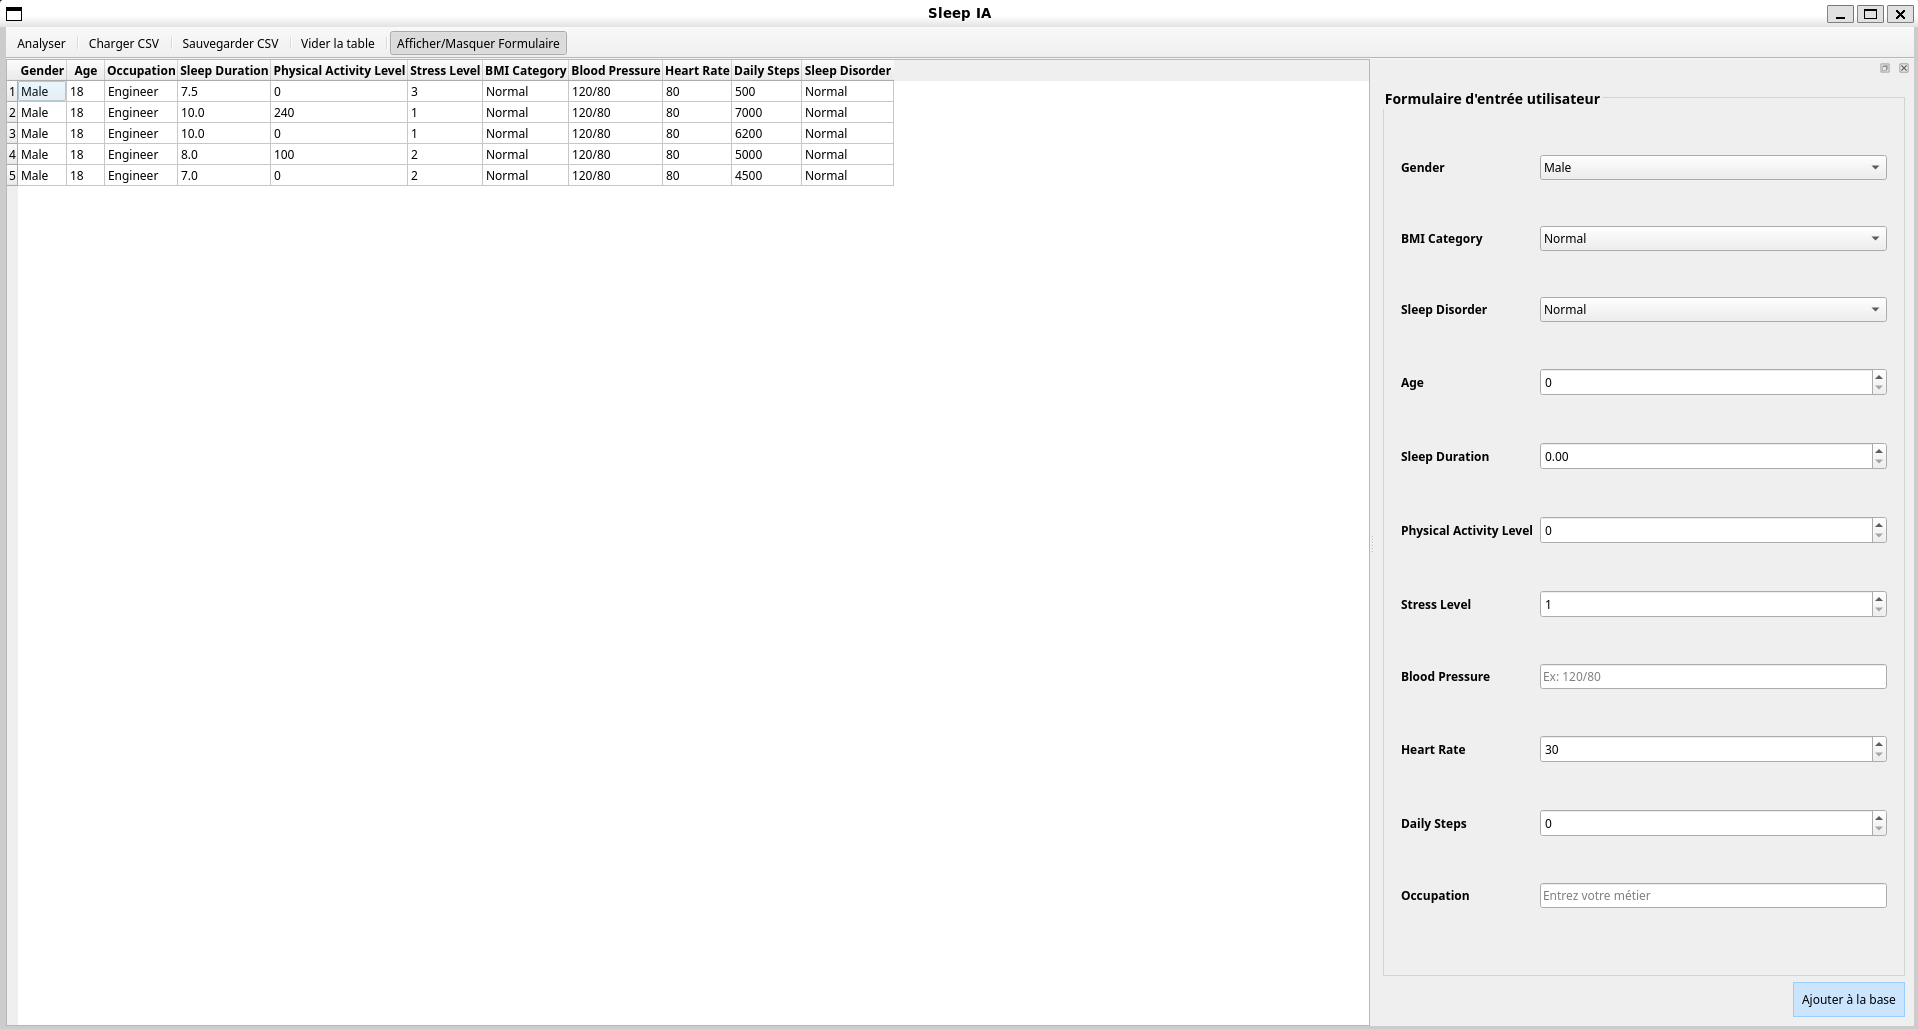
\includegraphics[width=0.7\textwidth]{screen_UI.png}
    % Capture d'écran de ton interface
  \end{center}
\end{frame}

\section{Discussion}

\begin{frame}{Limites et perspectives}
    \begin{block}{Données}
        Petit volume cause des imprécision et un déséquilibre de données
    \end{block}
    \begin{block}{Modèle}
         .....
    \end{block}
    \begin{block}{Pistes}
    \begin{itemize}
      \item Utilisation de séries temporelles
    \end{itemize}
    \end{block}
    
\end{frame}

\begin{frame}{Conclusion}
  \centering{\textit{Merci pour votre attention !}}
\end{frame}

\end{document}
